\section{Overall Description}
\subsection{Product Perspective}
\subsubsection{Scenarios}
\begin{enumerate}
    \item \textbf{Customer wants to start using the eMall service}\\
    The customer Matteo decides that he wants to use the eMall service to 
    take advantage of the efficiency it offers. 
    He launches the service and selects the option to sign up. 
    Matteo then inputs all the relevant information and he is granted access to the service.
    \item \textbf{Customer books the recharge for his car}\\
    After a long drive, the customer Matteo notices that the level of his battery is low. 
    He stops, takes his phone and launches the eMall service, logs in, and then he is presented with all the nearby stations.
    He selects different stations, checks their availability and views all the stations' information. The Customer then chooses a station according to his preferences and then finalizes the booking.
    He then receives the booking's summary, including the booked socket. He is also presented with a reminder that the booking will be kept for 15 minutes at most.
    \item \textbf{Customer starts the charge}\\
    The customer Matteo drives to a station that he has a charge booked with, he then unlocks the booked socket from the service, he then connects his electric 
    vehicle to the socket and, after he has left the vehicle, he launches the eMall service, navigates to his current booking, and 
    he is presented with the option to start the charge. He selects this option and the station initiates charging on the booked socket. eMall than shows the user the estimated time for the full charge of the vehicle. 
    \item \textbf{Customer is notified of a finished charge}\\
    After the customer Matteo has started to charging process at the station,
     he goes to a nearby cafeteria to have a cup of coffee. When the car has fully charge, the eMall service notifies him on his phone with a push notification.
    \item \textbf{Customer pays for the service}\\
    The customer Matteo, after he has used the eMall service for a successful charge and provided that he has not paid for the service yet,
    launches the app and he is presented with the option to pay for the service, 
    he selects this option and then enters his credit card information.
    The service that processes his payment, and if it is successful he is presented with a success message. The application will now mark that booking as paid.
    \item \textbf{Customer is reminded to charge his electric vehicle}\\
    While the customer Matteo is driving, the eMall service monitors the car's battery level, the customer's location and his schedule. 
    When the service finds an optimal place to charge, related to schedule, location and state of charge it notifies the customer with a push notification.
    Matteo then stops, launches the eMall service and then he is presented with the optimal station to charge, based on his location, his schedule and the stations' prices. He then books the charge.
    
    \item \textbf{CPO chooses from which DSO acquire energy}\\
    The CPO Evox wants to modify the DSO energy source of a charging station. The CPO's employee Mario launches the eMall service, logs in, and then through the dashboard he is able to select his first station and then selects the DSO MaDistribution from which to acquire energy.
    \item \textbf{CPO chooses the cost of a charging}\\
    The CPO Evox decides to modify the cost of a charging type in a specific station. The CPO's employee Mario launches the eMall service, logs in, and then using the dashboard selects the first station and then the charging type "fast", he then sets the charging price to 0.60€/kWh.    
    \item \textbf{CPO selects automatic cost calculation of a charging}\\
    The CPO Evox wants to set the automatic vehicle charging cost calculation. The CPO's employee Mario launches the eMall service, logs in, and then using the dashboard selects the first station and then the charging type "slow", he then set the charging price to automatic.      
    \item \textbf{CPO selects the battery policy discharge}\\
    The CPO Evox wants to change the battery usage policy, he wants to take half of the energy from the batteries and the other half from the DSO. The CPO's employee Mario launches the eMall service, logs in, and then using the dashboard select the second charging station and then set battery policy to discharge and the discharge factor to 50\%.
    \item \textbf{CPO select the battery policy disabled}\\
    The CPO Evox wants to disable the usage of batteries, neither to charge them neither to use them to charge the vehicles. The CPO's employee Mario launches the eMall service, logs in, and then using the dashboard selects the third charging station, and then set the battery policy to disabled.
    \item \textbf{CPO decides to make a special offer}\\
    The CPO Evox to promote his service decides to make a special 10\% discount on the price of fast charging in his second station. The CPO's employee Mario launches the eMall service, logs in, and then using the dashboard selects the station and the charging type. He set the offer percentage to 10\%

\end{enumerate}
\subsubsection{Class Diagram}
This is the Class Diagram of the system.
We consider the suggestion, that it's sent to the Customer via push notification, as a prepared booking. For this reason it inherits from the abstract class "BookingAbstract". The customer has to choose only if he wants to accept or not the suggested booking.
Assuming that every socket has a unique ID in the single station and charging stations have a unique ID too (w.r.t Domain Assumptions), the "Booking" class is associated both to the "Charging Station" and the "Socket" classes because it would be impossible to know the correspondent Charging station directly from the booked socket.


%\begin{figure}
 %   \hspace{-108px}
 %   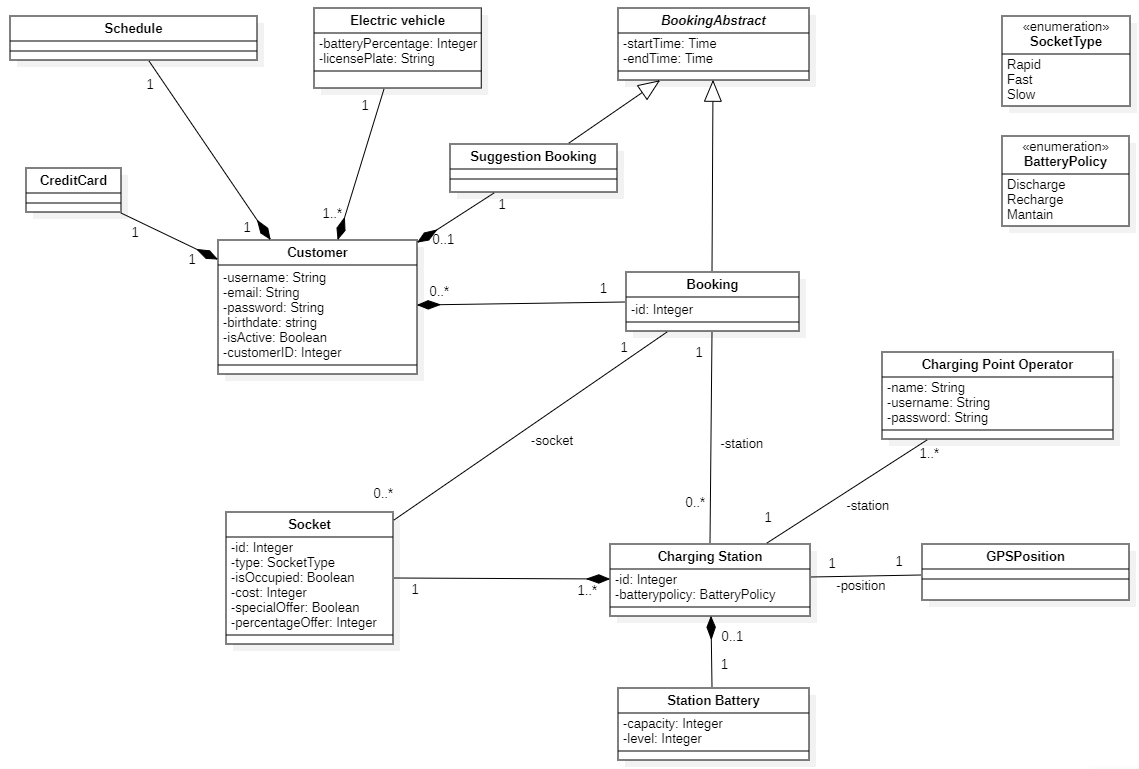
\includegraphics[scale=0.46]{img/UML_ClassDiagram.PNG}
 %   \caption{High-level UML diagram with main classes}
 %   \label{class_diagram}

%\end{figure}


%\subsubsection{State Diagrams}
\subsection{Product Functions}
In this section the main functionalities of eMall are presented and described.
\subsubsection{Sign up}
This functionality lets the registration of \textbf{Unregistered Customers}(\ref{Customer}) in order to use eMall. The first step is to enter the registration form, then the User inserts his credentials; if correct an e-mail is sent to the inserted address and it is required to validate it. 
Finally the User is taken to the login page.
\begin{figure}[H]
    \begin{center}
        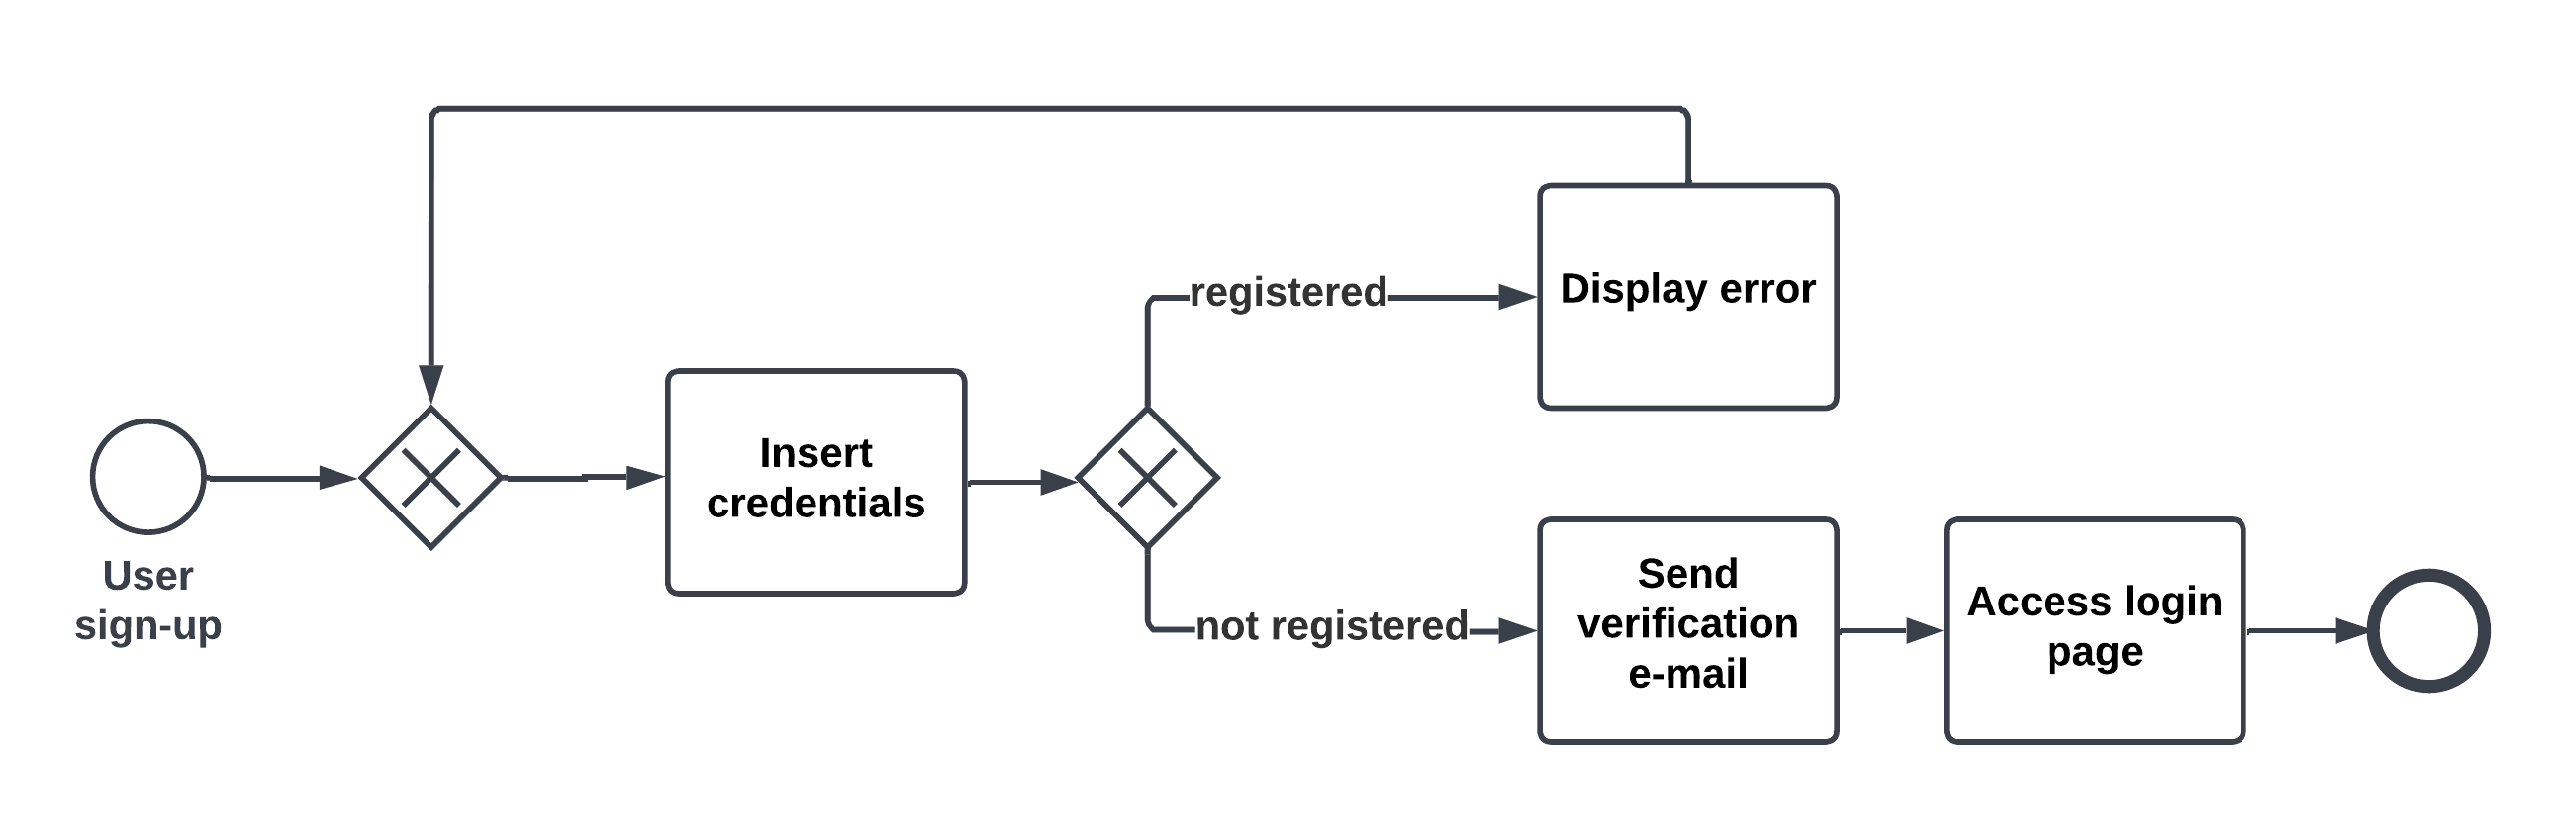
\includegraphics[width=\textwidth]{img/fun-sign-up.png}
        \caption{BPMN diagram sign up method}
    \end{center}
\end{figure}
\subsubsection{View the nearby charging stations}
This functionality allows the \textbf{Customers}(\ref{Customer}) to view information about the nearby charging stations, and is available to all of the logged Users. 
The first step is to open the eMall service and the User is presented with the nearby charging stations. 
If he clicks on one of the stations, the user can view the current station's recharge price and socket availability.
The User at any time can go back to view the other stations and he is free to view information about them.\label{View}
\begin{figure}[H]
    \begin{center}
        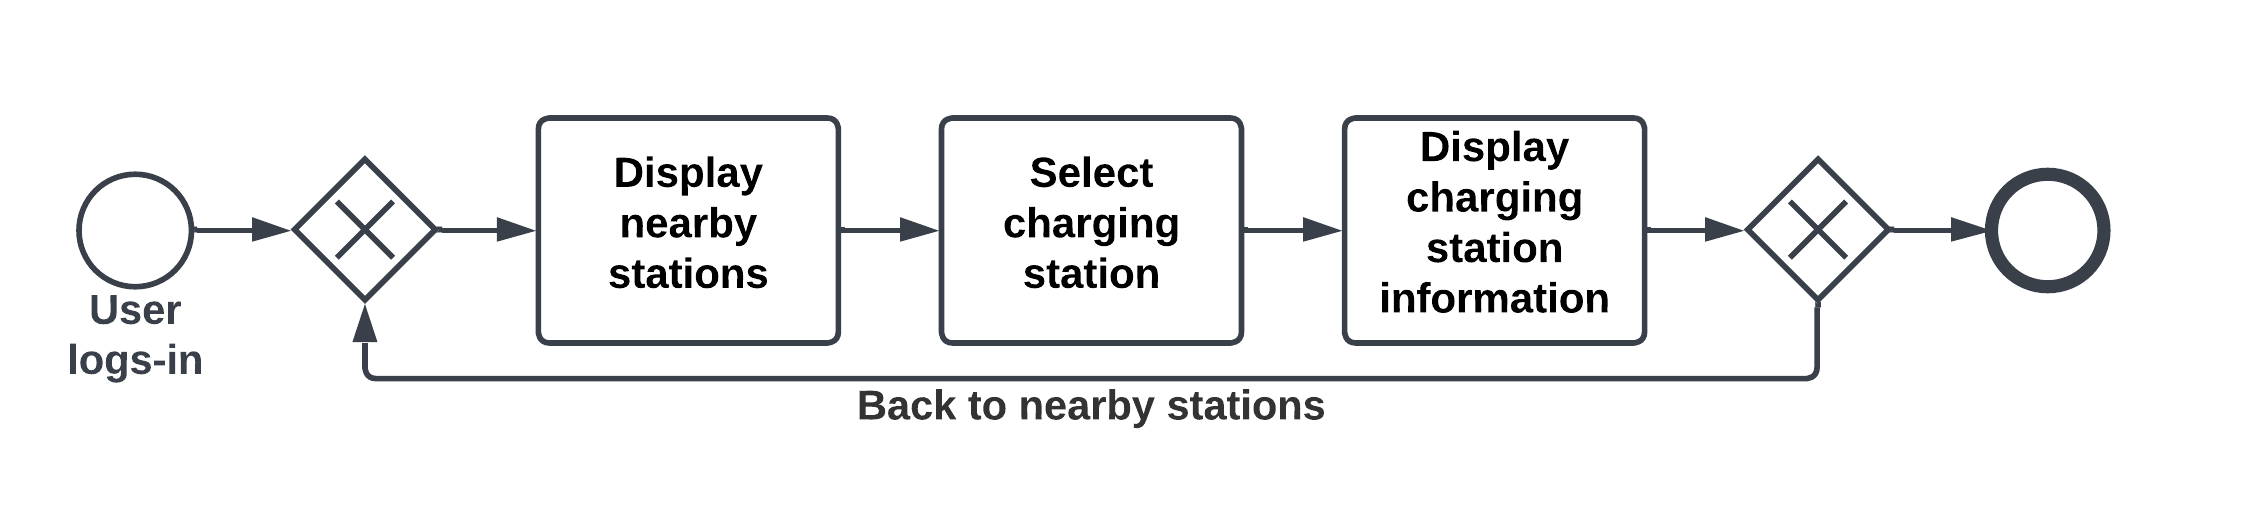
\includegraphics[width=\textwidth]{img/fun-view-info.png}
        \caption{BPMN diagram view nearby stations method}
    \end{center}
\end{figure}
\subsubsection{Charge booking}
This functionality allows the \textbf{Customers}(\ref{Customer}) to book a charge for their electric vehicle, and is available to all of the logged Users. 
The first step is to open the eMall service and to select a preferred timeslot for charging. The second step is to pick a station from the stations view (As described in \ref{View}).
Finally, the User can select the "Book" option to reserve his timeslot at the selected station for charging.
He then is presented with a brief summary of the booking, like the socket's identification and the station's address.
He can also view the summary at anytime in a specific section of the service.\label{Book} 
\begin{figure}[H]
    \begin{center}
        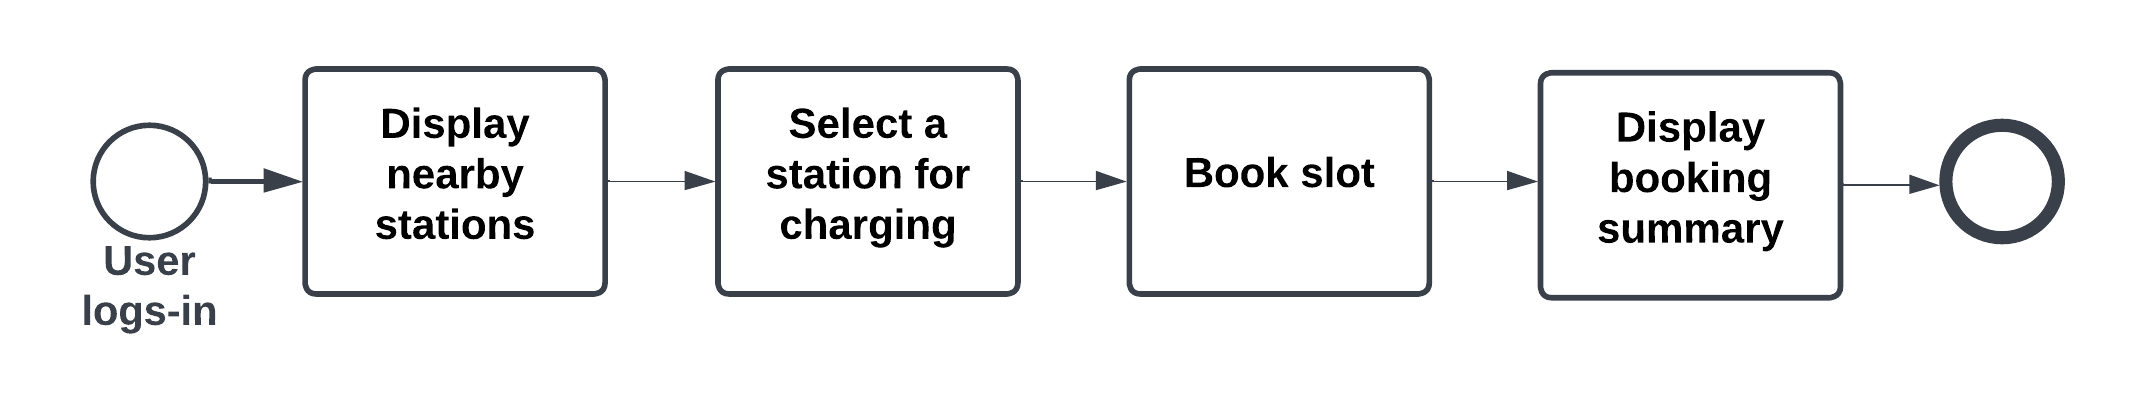
\includegraphics[width=\textwidth]{img/fun-book-slot.png}
        \caption{BPMN diagram charge booking method}
    \end{center}
\end{figure}
\subsubsection{Remotely unlocking a socket}
This functionality allows the \textbf{Customers}(\ref{Customer}) to unlock a charging socket to charge their electric vehicle, and is available when a logged User has booked a recharge at a station. 
The User must access the brief summary of his booking (As described in \ref{Book}).
He can select the "Unlock" option to unlock his booked socket, in order to connect his car to the socket.
\begin{figure}[H]
    \begin{center}
        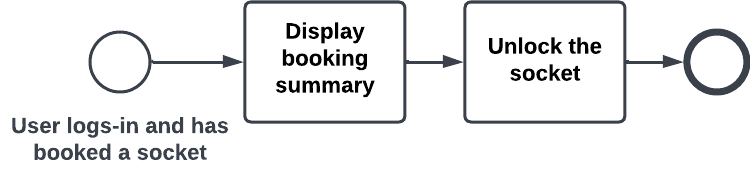
\includegraphics[scale=0.3]{img/fun-sock-unl.png}
        \caption{BPMN diagram socket unlocking method}
    \end{center}
\end{figure}
\subsubsection{Remotely starting a charge}
This functionality allows the \textbf{Customers}(\ref{Customer}) to remotely start the charge for their electric vehicle, and is available when a logged User has booked a recharge at a station, and has connected his car to the socket. 
The User must access the brief summary of his booking (As described in \ref{Book}).
He can select the "Start charging" button to remotely start the charging process on his booked socket.
\begin{figure}[H]
    \begin{center}
        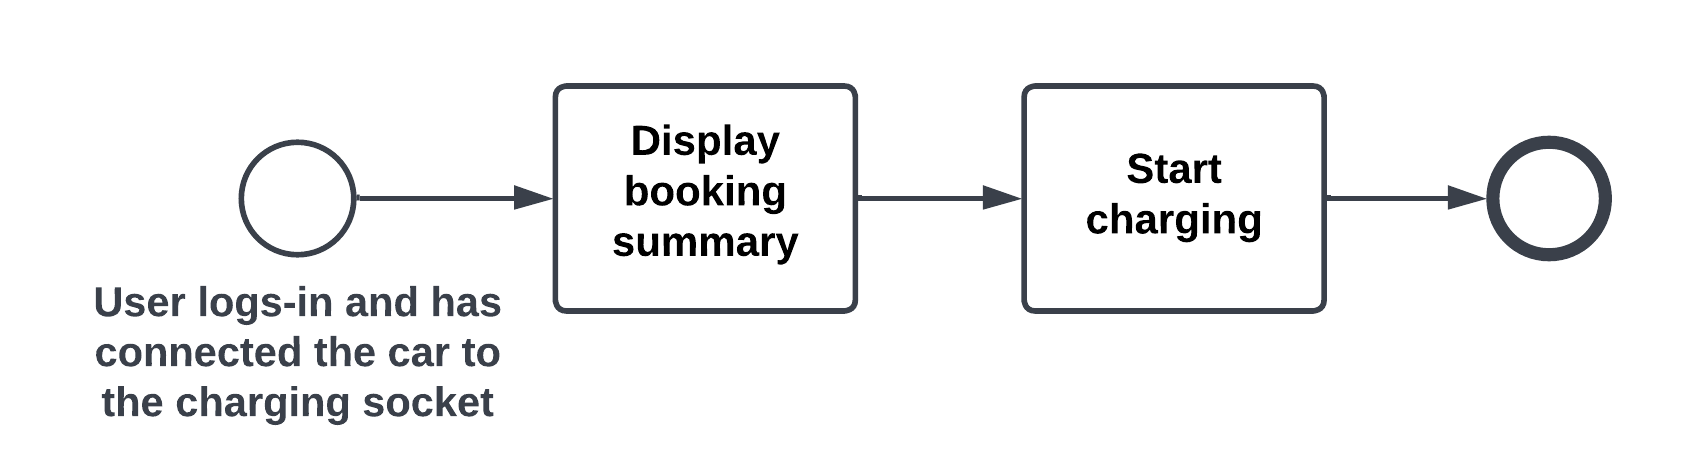
\includegraphics[scale=0.2]{img/fun-rem-ch.png}
        \caption{BPMN diagram remotely starting the charge method}
    \end{center}
\end{figure}
\subsubsection{Notify of a finished charge}
This functionality allows the \textbf{Customers}(\ref{Customer}) to be informed when the charging process has finished, and is available when a logged User has been charging his car at a station.
When the charging process ends, the user is notified (with a push notification) that his car is fully charged.
\begin{figure}[H]
    \begin{center}
        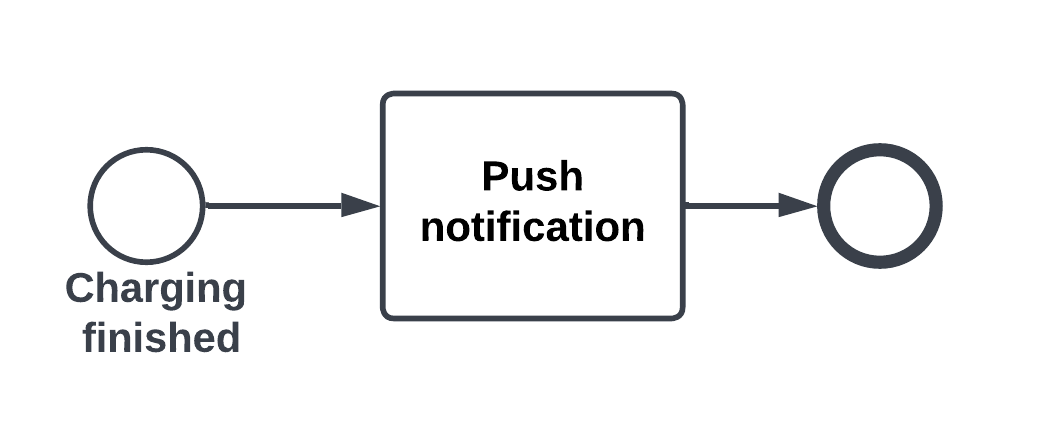
\includegraphics[scale=0.2]{img/fun-not-fin.png}
        \caption{BPMN diagram notify a finished charge method}
    \end{center}
\end{figure}
\subsubsection{Pay for the service}
This functionality allows the \textbf{Customers}(\ref{Customer}) to pay for the charging service, provided that he has used the service.
When the charging process ends, the User can open the brief summary of his reservation (As described in \ref{Book}) in order to pay for the service.
After the opens the summary, he is presented with the option to pay and if it picked, he should enter his credit card's information and click the "Submit" button.
If the payment has been successful, the service shows him the success screen and the summary of the reservation will be marked as paid, otherwise he is returned to enter a valid credit card's information.
\begin{figure}[H]
    \begin{center}
        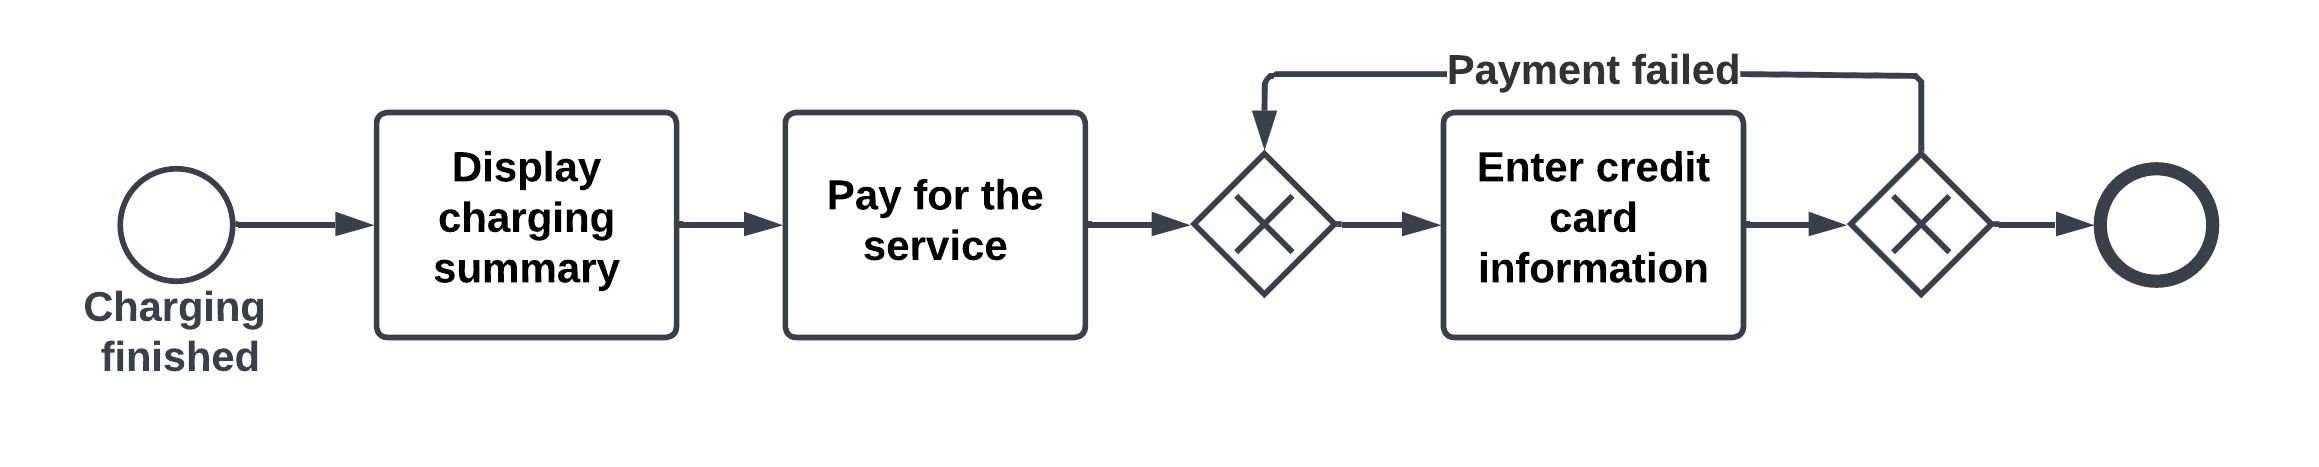
\includegraphics[width=\textwidth]{img/fun-pay.png}
        \caption{BPMN diagram pay for the service method}
    \end{center}
\end{figure}
\subsubsection{Send suggestions}
This functionality allows the \textbf{Customer}(\ref{Customer}) to receive optimal suggestions for charging.
The system continously monitors a user's charging level, his schedule and his location.
The system has an internal model to determine an optimal place to charge if battery level is under 50\%, based on location and schedule.
When it determines an optimal place and timeslot, the model will also determine the optimal time to suggest the user.
The user will than be notified at the computed time with a push notification. The notification will contain the optimal place to charge and an optimal timeslot, with maximum compatibility with the user's lifestyle. 
\begin{figure}[H]
    \begin{center}
        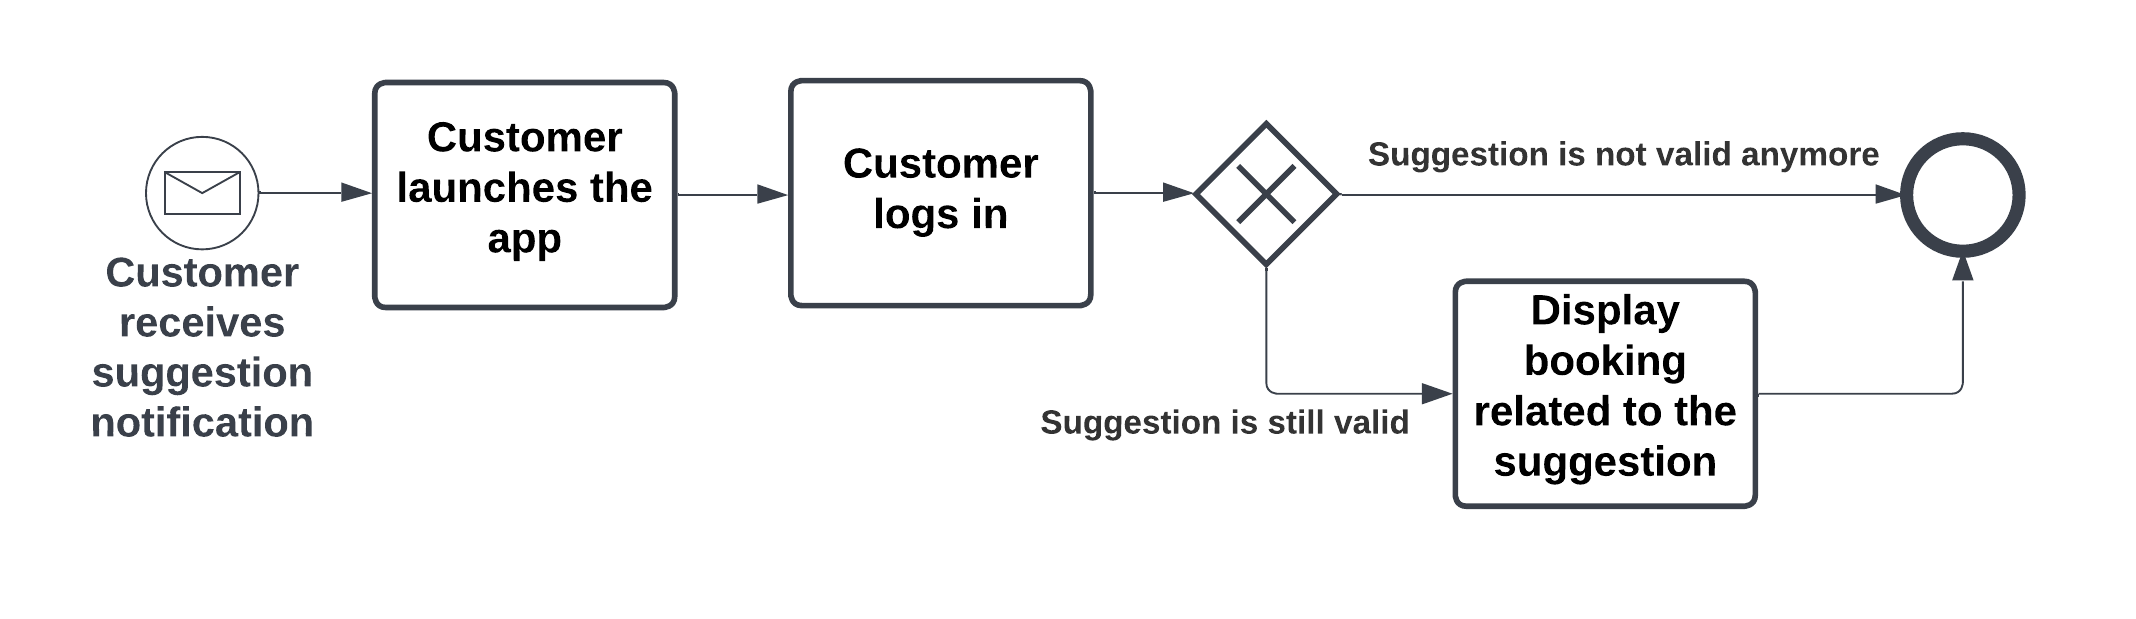
\includegraphics[width=\textwidth]{img/fun-sug.png}
        \caption{BPMN diagram send suggestions method}
    \end{center}
\end{figure}
\subsubsection{Select the charging station's energy provider}
This functionality allows the \textbf{CPOs}(\ref{CPO}) to manually adjust the energy provider. An energy provider can be select automatically or a CPO can manually select a specific \textbf{DSO}\ref{DSO}) for the supply of energy. The first step for the CPO is to log in in the platform and select a charging station. Then, the CPO can select an energy provider option for the station.
\begin{figure}[H]
    \begin{center}
        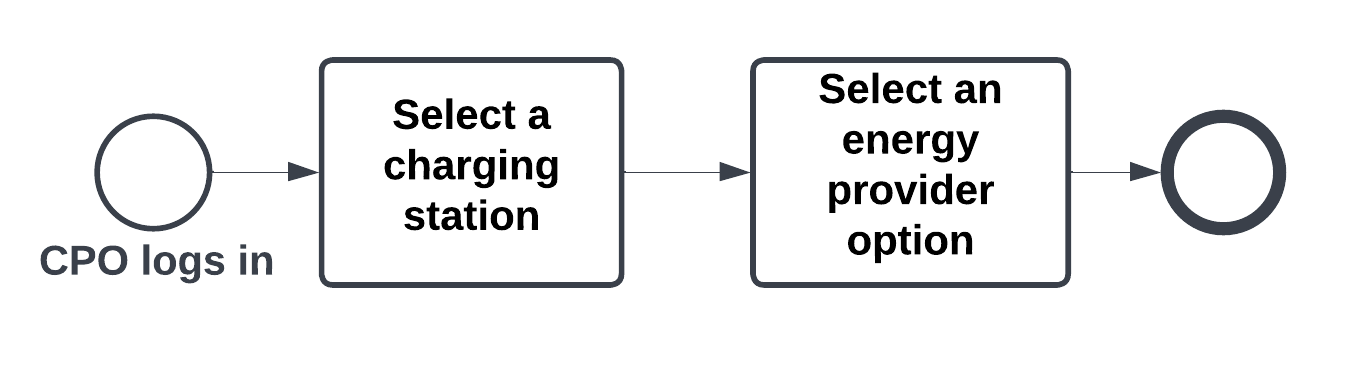
\includegraphics[width=\textwidth]{img/fun-en-prov.png}
        \caption{BPMN diagram select energy provider method}
    \end{center}
\end{figure}
\subsubsection{Select a battery policy for a charging station}
This functionality allows the \textbf{CPOs}(\ref{CPO}) to manualy select a battery policy for a charging station. A battery policy can be automatically select, or a charge, discharge and disable policy can be selected. The first step for the CPO is to log in in the platform and select a charging station. Then, the CPO can select a battery policy. If the discharge policy is selected, a CPO can also select a discharging factor, that will determine how much energy from the batteries will be mixed with the energy from the \textbf{DSOs}\ref{DSO}.
\begin{figure}[H]
    \begin{center}
        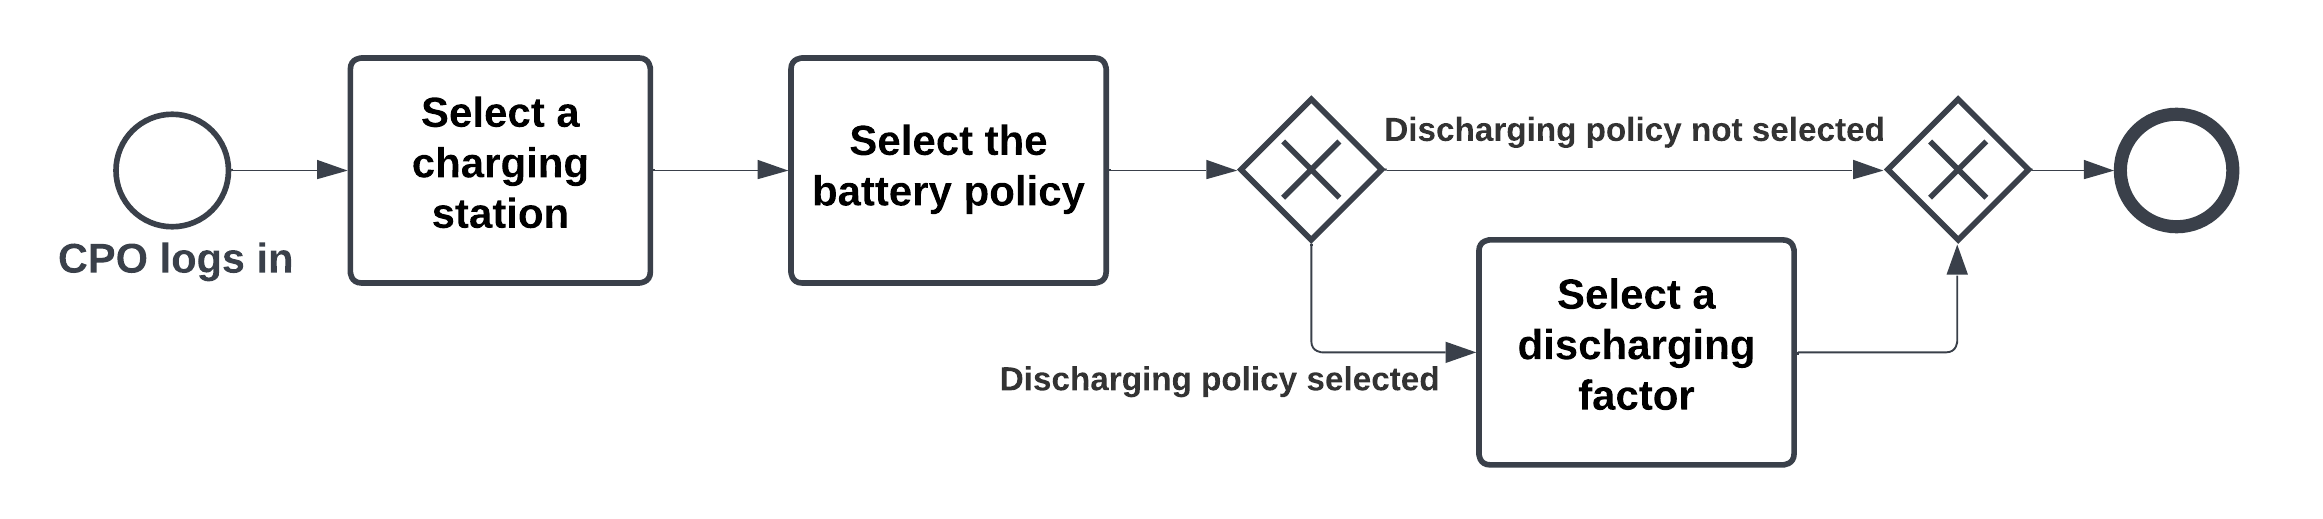
\includegraphics[width=\textwidth]{img/fun-bat-pol.png}
        \caption{BPMN diagram select battery policy method}
    \end{center}
\end{figure}
\subsubsection{Select the charging station's charging cost}
This functionality allows the \textbf{CPOs}(\ref{CPO}) to manually adjust the charging price at a station. The first step for the CPO is to log in in the platform and select a charging station. The second step is to select a specific charging type, such as slow, fast and rapid. Finally, the CPO can select a charging cost. Also, an option is present to apply a special offer (in percentage) on the current charging cost.
\begin{figure}[H]
    \begin{center}
        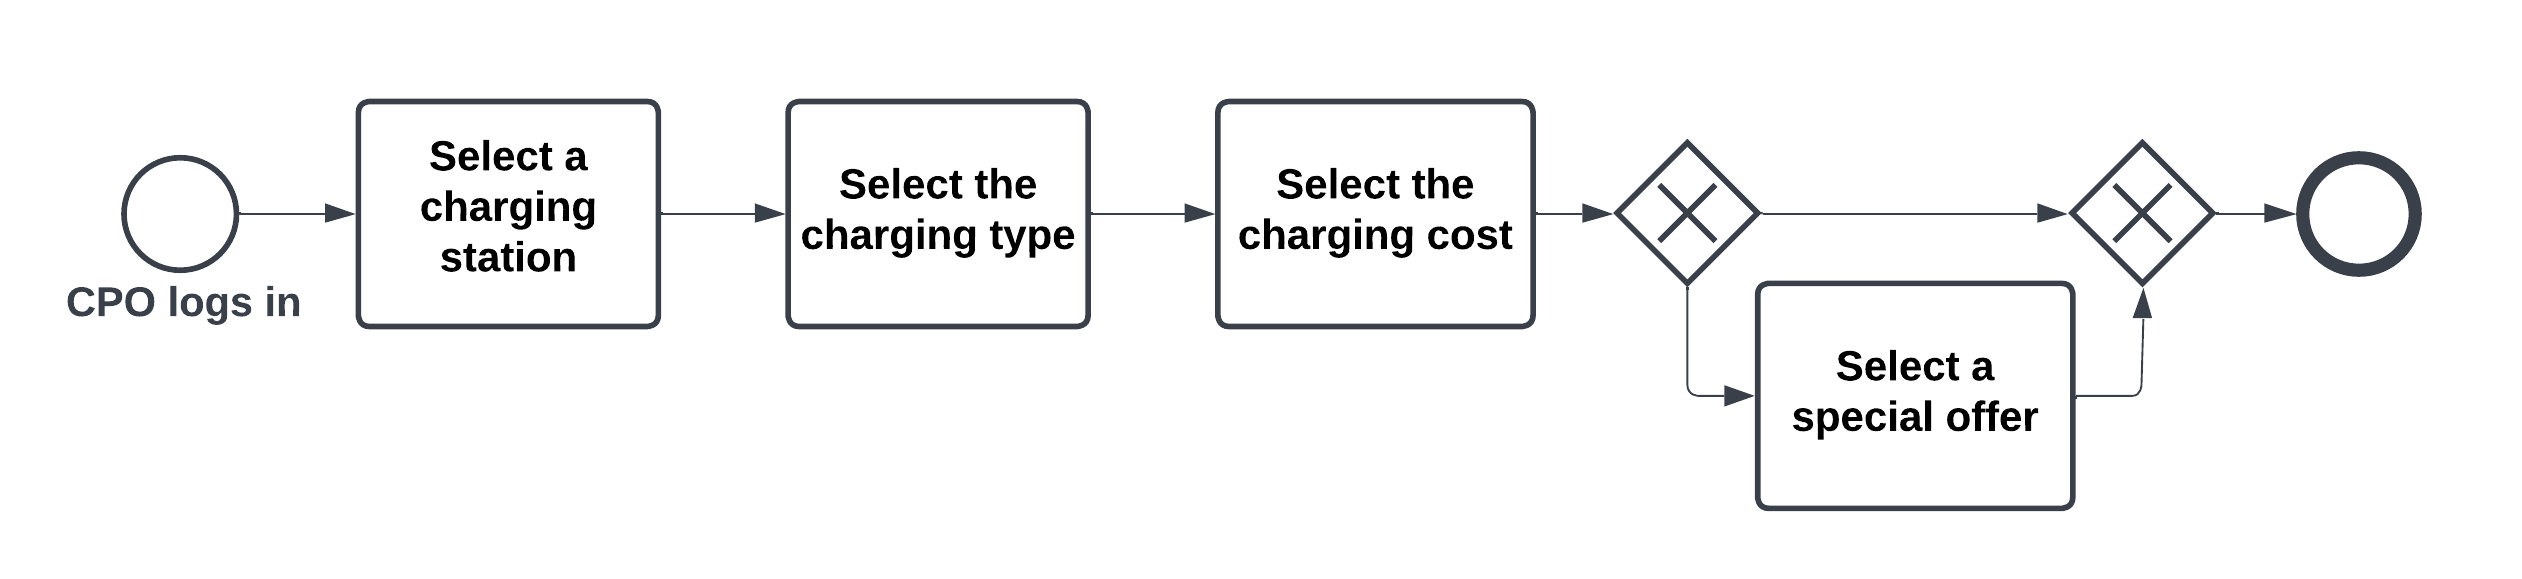
\includegraphics[width=\textwidth]{img/fun-char-cost.png}
        \caption{BPMN diagram send suggestions method}
    \end{center}
\end{figure}
%
\subsection{User Characteristics}
The following three actors are considered in the e-Mall system.
\subsubsection{Unregistered Customer}
It's a person that doesn't have a registered account in the e-Mall application. 
In this case, he can register an account to use the platform.
\subsubsection{Registered Customer}
It's a person that has a registered account in the e-Mall application. 
He is able to use the e-Mall service and book a charge for his electric vehicle through the service.
He is also able to unlock a charging socket for his reservation and to pay for the service through the platform.
\subsubsection{Charging Point Operator}
It's the charging station owner and manager. This actor is responsible for the supply of the charging service offered by eMSP. 
Every reservation made on the e-Mall platform is fulfilled by CPOs.
\subsection{Assumptions, Dependencies and Constraints}
\subsubsection{Domain assumptions}
\begin{enumerate}[label=\textbf{D\arabic*}:]
    \item Each user who wants to use eMall needs to have a mobile device with the most common mobile OSes (e.g. iOS, Android), and also a reliable Internet connection with that device.
    \item Each CPO who wants to access the CPMS platform needs to have a device connected to the Internet (such as PC, Mac, smartphone, etc), with the most common Web Browsers (e.g. Firefox, Google Chrome, Microsoft Edge, Apple Safari, etc).  
    \item The customer's mobile device fully supports the push notification technology.
    \item The customer's schedule and location is accessible by the platform.
    \item The charging station checks the charging sockets, making sure that nobody can occupy a reserved socket apart from the booker.
    \item The data automatically obtained by the system in order to send suggestions to the user is accurate and truthful.
    \item Every CPMS system has the same communication methods. (Uniform APIs)
    \item A fully functioning payment system is present and returns if a transaction has been successful or not.
    \item Every station has at least one charging socket.**
    \item Every eMSP must interact with at least one CPO.**
    \item Every CPO is supplied with login credentials when the system is installed.
    \item Every Charging Station has a unique identification number (ID).
    \item Sockets in each station have a unique identification number (ID). Sockets in different charging stations could have the same ID.
    \item Given a license plate number and personal identification, it exists an API that provides the battery level of the vehicle associated with the license plate.
    \item All the sockets present in charging stations feature a system that can retrieve the charging level of a car after it has been connected to the socket.
\end{enumerate}